\part{Traveling Salesman Problem}
\chapter{Symmetric Traveling Salesman Problem}
旅行商问题(Traveling Salesman Problem, TSP\index{TSP})是组合优化领域的经典问题之一,其核心目标是给定城市列表和每对城市之间的距离,求恰好访问每个城市一次并返回起始城市的最短可能路线。该问题于1930年正式提出,是优化中研究最深入的问题之一,被用作许多优化方法的基准。自从该问题被正式提出以来,一直是运筹学、计算机科学和物流管理等领域的研究热点,尽管该问题在计算上很困难,但许多启发式方法和精确算法是已知的\cite{2009A, 2012Models}。

\begin{figure}[!htb]
    \centering
    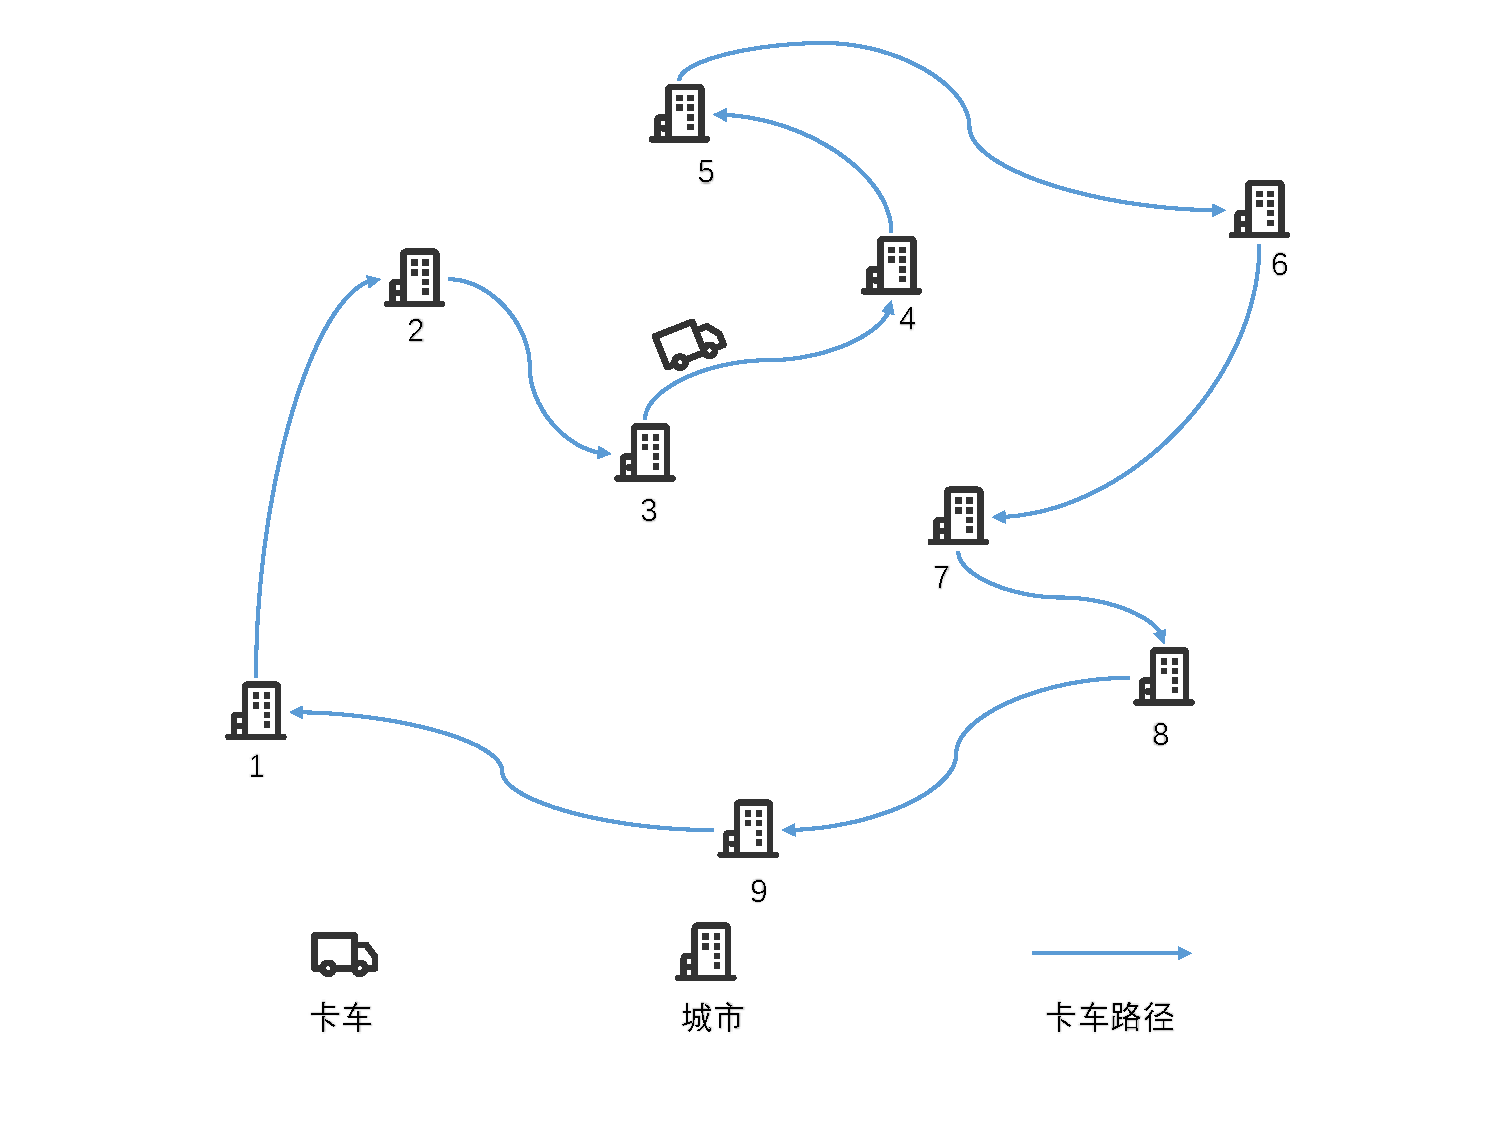
\includegraphics[width=\linewidth]{images/TSP.pdf}\\
    \caption{TSP示意图}
\end{figure}

TSP可以表述为整数线性规划模型\cite{papadimitriou1998combinatorial}:假设共有$N$个城市,每个城市的编号为$1,\cdots,N$,从城市$i$到城市$j$的旅行成本(距离)为$c_{ij}>0$。旅行商的目标是从任意一个城市出发访问完所有的城市,每个城市只能访问一次,最后回到最初的城市,目标是找到一条依次访问所有城市且访问城市不重复的最短路线。TSP中的决策变量为$x_{ij}=\begin{cases}1, & \text{存在从城市$i$到城市$j$的路径}\\0, & \text{其他} \end{cases}$,城市节点集合表示为$V(|V| = N)$。由于可能存在子回路,所以在构建TSP模型时需要消除会产生子回路的情况,这里采用Miller-Tucker-Zemlin (MTZ\index{MTZ})约束进行子回路的消除\cite{1960Integer},引入连续变量$u_i(\forall i \in V, u_i \geq 0)$,其取值可以为任何非负实数(实数集合表示为$R$)。这里用$u_i$表示编号为$i$的城市的访问次序,比如当$u_i = 5$时表示编号为1的城市是从出发点开始,第5个被访问到的点。因此,TSP的数学模型可以表示为MILP \ref{model:model-tsp}。

\begin{model}{TSP MILP}{model-tsp}
\begin{align}
    \min \quad & \sum_{i \in V}\sum_{j \in V, i \neq j} c_{ij}x_{ij} & \label{eq:tsp-obj}\\
    \text{s.t.} \quad & \sum_{i \in V} x_{ij} = 1, & \forall j \in V, i \neq j\label{eq:tsp-in}\\
    \quad & \sum_{j \in V} x_{ij} = 1, & \forall i \in V, i \neq j \label{eq:tsp-out}\\
    \quad & u_i - u_j + Nx_{ij} \leq N - 1, & \forall i, j \in V; i \neq j \label{eq:tsp-subtour}\\
    \quad & u_i \geq 0, & u_i \in R \label{eq:tsp-u_bound}\\
    \quad & x_{ij} \in \{0, 1\}, & i, j \in V; i \neq j\label{eq:tsp-x_bound}
\end{align}
\end{model}

目标函数\ref{eq:tsp-obj}表示最小化访问所有城市的成本(距离),约束\ref{eq:tsp-in}和\ref{eq:tsp-out}保证每个城市节点的入度和出度为1,即每个城市只进入一次和出去一次,保证了每个城市只访问一次,不会被重复访问,约束\ref{eq:tsp-subtour}消除子回路,约束\ref{eq:tsp-u_bound}和\ref{eq:tsp-x_bound}表示变量的取值范围。
